\section{Implications of the periodic boundary condition}
\dfn{Amount of allowed $\vec{k}$-states, N}{
	The amount of allowed $\vec{k}$-states, N, is given by the amount of unit cells that build the crystal. This implicates that in each energy band $E_n(\vec{k})$, where $\vec{k} \in$ first BZ, there are N allowed $\vec{k}$-states.
}

There are serveral cases we can study, we will go over them.

\subsection{Case 1 - N is odd}
Take the amount of valence electrons in each unit cell is odd. If we consider the first BZ we get the energy band structure that is given in figure \ref{fig:N_odd_band_struct}. For each $\vec{k}$-state, we can have two electrons: spin up and spin down. Ìn this picture, the circles decpict a hole. Furthermore, the temperature in this figure is $0K$, all electrons are in their base state.\par
Now, the fact that we have an odd number of electrons, we need to have partially filled bands. In this case we have metallic crystals.
\begin{figure}[h]
	\centering
	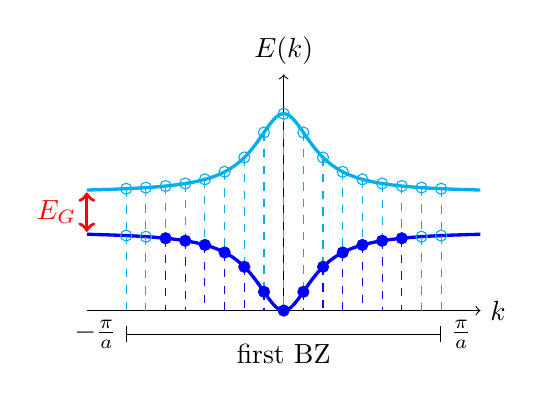
\begin{tikzpicture}[domain=-2.5:2.5]
		\draw[->] (-2.5,0) -- (2.5,0) node[right] {$k$};
		\draw[->] (0,0) -- (0, 3) node[above] {$E(k)$};

		\draw[blue, very thick] plot[samples=200] (\x, {1 - 1/(1 + 5*\x*\x)});
		\draw[cyan, very thick] plot[samples=200] (\x, {1.5 + 1/(1 + 5*\x*\x)});

		\draw[<->, red, very thick]	(-2.5, 1) to node[left]{$E_G$} (-2.5, 1.5);

		\foreach \x in {-8,...,8} {
			\draw[cyan]	({\x / 4}, {1.5 + 1/(1 + 5*\x*\x / 16)}) circle (2pt);
			\draw[dashed, cyan]	({\x / 4}, {1.5 + 1/(1 + 5*\x*\x / 16)}) to ({\x / 4}, {1 - 1/(1 + 5*\x*\x / 16)});
		}

		\foreach \x in {-8,...,8} {
			\ifnum \x < -6 {
				\draw[cyan]	({\x / 4}, {1 - 1/(1 + 5*\x*\x / 16)}) circle (2pt);
				\draw[dashed, cyan]	({\x / 4}, {1 - 1/(1 + 5*\x*\x / 16)}) to ({\x / 4}, 0);
			}
			\else {
				\ifnum \x > 6 {
					\draw[cyan]	({\x / 4}, {1 - 1/(1 + 5*\x*\x / 16)}) circle (2pt);
					\draw[dashed, cyan]	({\x / 4}, {1 - 1/(1 + 5*\x*\x / 16)}) to ({\x / 4}, 0);
				}
				\else {
					\filldraw[blue]	({\x / 4}, {1 - 1/(1 + 5*\x*\x / 16)}) circle (2pt);
					\draw[dashed, blue]	({\x / 4}, {1 - 1/(1 + 5*\x*\x / 16)}) to ({\x / 4}, 0);
				} \fi
			} \fi
		}

		\draw	(-2, -0.3)	node[left]{$-\frac{\pi}{a}$};
		\draw	(2, -0.3)	node[right]{$\frac{\pi}{a}$};

		\draw[|-|]	(-2, -0.3) to node[below]{first BZ} (2, -0.3);
	\end{tikzpicture}
	\caption{Band structure with odd number of electrons}
	\label{fig:N_odd_band_struct}
\end{figure}
\subsection{Case 2 - N is even}
The amount of electrons in each unit cell is even. Again, we consider the first BZ. We get figure \ref{fig:N_even_band_struct}. Now we speak about a semiconductor (or an insulator if $E_G$ is large).
\begin{figure}[h]
	\centering
	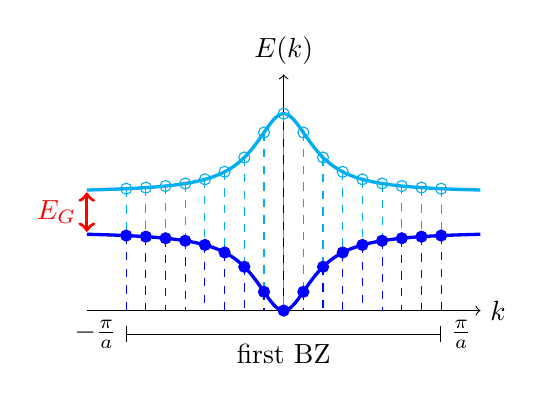
\begin{tikzpicture}[domain=-2.5:2.5]
		\draw[->] (-2.5,0) -- (2.5,0) node[right] {$k$};
		\draw[->] (0,0) -- (0, 3) node[above] {$E(k)$};

		\draw[blue, very thick] plot[samples=200] (\x, {1 - 1/(1 + 5*\x*\x)});
		\draw[cyan, very thick] plot[samples=200] (\x, {1.5 + 1/(1 + 5*\x*\x)});

		\draw[<->, red, very thick]	(-2.5, 1) to node[left]{$E_G$} (-2.5, 1.5);

		\foreach \x in {-8,...,8} {
			\draw[cyan]	({\x / 4}, {1.5 + 1/(1 + 5*\x*\x / 16)}) circle (2pt);
			\draw[dashed, cyan]	({\x / 4}, {1.5 + 1/(1 + 5*\x*\x / 16)}) to ({\x / 4}, {1 - 1/(1 + 5*\x*\x / 16)});
		}

		\foreach \x in {-8,...,8} {
			\filldraw[blue]	({\x / 4}, {1 - 1/(1 + 5*\x*\x / 16)}) circle (2pt);
			\draw[dashed, blue]	({\x / 4}, {1 - 1/(1 + 5*\x*\x / 16)}) to ({\x / 4}, 0);
		}

		\draw	(-2, -0.3)	node[left]{$-\frac{\pi}{a}$};
		\draw	(2, -0.3)	node[right]{$\frac{\pi}{a}$};

		\draw[|-|]	(-2, -0.3) to node[below]{first BZ} (2, -0.3);
	\end{tikzpicture}
	\caption{Band structure with odd number of electrons}
	\label{fig:N_even_band_struct}
\end{figure}
\subsection{Case 3 - N is even + band overlap}
The amount of electrons in the crystal is even and we have a band overlap. We now get a figure as figure \ref{fig:N_even_band_struct_w_overlap}. As you might guess, we get a metal again. Because now the electrons can move in their energyband when an electric field is applied.
\begin{figure}[h]
	\centering
	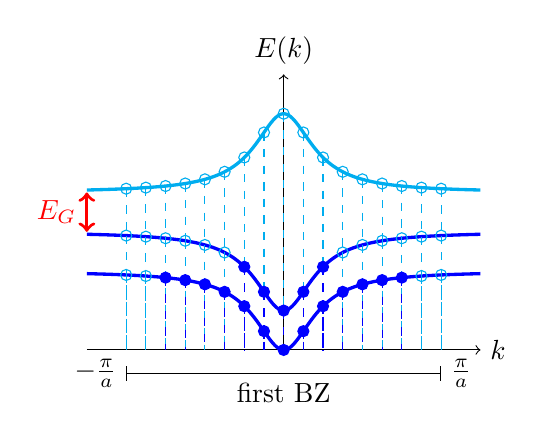
\begin{tikzpicture}[domain=-2.5:2.5]
		\draw[->] (-2.5,0) -- (2.5,0) node[right] {$k$};
		\draw[->] (0,0) -- (0, 3.5) node[above] {$E(k)$};

		\draw[blue, very thick] plot[samples=200] (\x, {1 - 1/(1 + 5*\x*\x)});
		\draw[blue, very thick] plot[samples=200] (\x, {1.5 - 1/(1 + 5*\x*\x)});
		\draw[cyan, very thick] plot[samples=200] (\x, {2 + 1/(1 + 5*\x*\x)});

		\draw[<->, red, very thick]	(-2.5, 1.5) to node[left]{$E_G$} (-2.5, 2);

		\foreach \x in {-8,...,8} {
			\draw[cyan]	({\x / 4}, {2 + 1/(1 + 5*\x*\x / 16)}) circle (2pt);
			\draw[dashed, cyan]	({\x / 4}, {2 + 1/(1 + 5*\x*\x / 16)}) to ({\x / 4}, {1.5 - 1/(1 + 5*\x*\x / 16)});
		}

		\foreach \x in {-8,...,8} {
			\ifnum \x < -2 {
				\draw[cyan]	({\x / 4}, {1.5 - 1/(1 + 5*\x*\x / 16)}) circle (2pt);
				\draw[dashed, cyan]	({\x / 4}, {1.5 - 1/(1 + 5*\x*\x / 16)}) to ({\x / 4}, 0);
			}
			\else {
				\ifnum \x > 2 {
					\draw[cyan]	({\x / 4}, {1.5 - 1/(1 + 5*\x*\x / 16)}) circle (2pt);
					\draw[dashed, cyan]	({\x / 4}, {1.5 - 1/(1 + 5*\x*\x / 16)}) to ({\x / 4}, 0);
				}
				\else {
					\filldraw[blue]	({\x / 4}, {1.5 - 1/(1 + 5*\x*\x / 16)}) circle (2pt);
					\draw[dashed, blue]	({\x / 4}, {1.5 - 1/(1 + 5*\x*\x / 16)}) to ({\x / 4}, 0);
				} \fi
			} \fi
		}

		\foreach \x in {-8,...,8} {
			\ifnum \x < -6 {
				\draw[cyan]	({\x / 4}, {1 - 1/(1 + 5*\x*\x / 16)}) circle (2pt);
				\draw[dashed, cyan]	({\x / 4}, {1 - 1/(1 + 5*\x*\x / 16)}) to ({\x / 4}, 0);
			}
			\else {
				\ifnum \x > 6 {
					\draw[cyan]	({\x / 4}, {1 - 1/(1 + 5*\x*\x / 16)}) circle (2pt);
					\draw[dashed, cyan]	({\x / 4}, {1 - 1/(1 + 5*\x*\x / 16)}) to ({\x / 4}, 0);
				}
				\else {
					\filldraw[blue]	({\x / 4}, {1 - 1/(1 + 5*\x*\x / 16)}) circle (2pt);
					\draw[dashed, blue]	({\x / 4}, {1 - 1/(1 + 5*\x*\x / 16)}) to ({\x / 4}, 0);
				} \fi
			} \fi
		}

		\draw	(-2, -0.3)	node[left]{$-\frac{\pi}{a}$};
		\draw	(2, -0.3)	node[right]{$\frac{\pi}{a}$};

		\draw[|-|]	(-2, -0.3) to node[below]{first BZ} (2, -0.3);
	\end{tikzpicture}
	\caption{Band structure with odd number of electrons}
	\label{fig:N_even_band_struct_w_overlap}
\end{figure}

\section{Calculating the band structre & solving for the bandstructure}
How do we get the bands? By just calculating the Schödinger equations, of course. Remember we did this for a free electron in section \ref{sec:nearly_free_e_approx}. There, we solved the equation:
\begin{equation}
	\left[-\frac{\hbar^2}{2m}\nabla^2 + V(\vec{r})\right]\psi_{n, \vec{k}}(\vec{r}) = E_n(\vec{k})\psi_{n, \vec{k}}(\vec{r})
\end{equation}
There are also other methods, i.e., the Tight Binding approach. This method is more representative for the band diagrams drawn in section \ref{sec:atomic_picture}. In the Tight Binding approximation, one writes the atomic and electronic part seperatly, which leads to solving the above Schrödinger equation in terms of atomic orbitals. The atomic orbitals are the ones we have drawn in section \ref{sec:atomic_picture}.\par
The prediction of the atomic orbitals, as given in section \ref{sec:atomic_picture}, cannot be predicted with the nearly free electron approximation. In this approximation, it seems as if all orbitals are s-orbitals. Where both Tight Binding and Nearly Free electron approximation do predict right is the placement of the bandgap, which is at the Bragg-points.
